\documentclass[letterpaper, 10 pt, conference]{ieeeconf}  % Comment this line out if you need a4paper
%\documentclass[a4paper, 10pt, conference]{ieeeconf}      % Use this line for a4 paper

\IEEEoverridecommandlockouts                              % This command is only needed if
                                                          % you want to use the \thanks command

\overrideIEEEmargins                                      % Needed to meet printer requirements.

% \pdfobjcompresslevel=0
% \pdfminorversion=4

\usepackage{graphicx} % for pdf, bitmapped graphics files
\usepackage{times} % assumes new font selection scheme installed
\usepackage{amsmath} % assumes amsmath package installed
\usepackage{amssymb}  % assumes amsmath package installed
\usepackage{bbold}
\usepackage{url}
\usepackage{cite}
\usepackage{enumerate}
\usepackage{booktabs}
\usepackage{tabularx}
\usepackage{multirow}
\usepackage{pifont}
\usepackage[table,xcdraw]{xcolor}
\usepackage{xspace}
\usepackage{float} % here for H placement parameter

\makeatletter
\let\NAT@parse\undefined
\makeatother
\usepackage[pagebackref=false,breaklinks=true,letterpaper=true,colorlinks,bookmarks=false]{hyperref}

% \usepackage[hidelinks]{hyperref} %hide the borders of the cross-references

\definecolor{baselinecolor}{gray}{.9}
\newcommand{\baseline}[1]{\cellcolor{baselinecolor}{#1}}
\newcommand{\fadedtext}[1]{\textcolor{gray}{#1}}


\newcolumntype{x}[1]{>{\centering\arraybackslash}p{#1pt}}
\newcolumntype{y}[1]{>{\raggedright\arraybackslash}p{#1pt}}
\newcolumntype{z}[1]{>{\raggedleft\arraybackslash}p{#1pt}}
\newlength\savewidth\newcommand\shline{\noalign{\global\savewidth\arrayrulewidth
\global\arrayrulewidth 1pt}\hline\noalign{\global\arrayrulewidth\savewidth}}
\newcommand{\tablestyle}[2]{\setlength{\tabcolsep}{#1}\renewcommand{\arraystretch}{#2}\centering\footnotesize}
\renewcommand{\paragraph}[1]{\vspace{1.25mm}\noindent\textbf{#1}}

\newcommand{\cmark}{\ding{51}}%
\newcommand{\xmark}{\ding{55}}%

\makeatletter
\DeclareRobustCommand\onedot{\futurelet\@let@token\@onedot}
\def\@onedot{\ifx\@let@token.\else.\null\fi\xspace}
\def\eg{\emph{e.g}\onedot} \def\Eg{\emph{E.g}\onedot}
\def\ie{\emph{i.e}\onedot} \def\Ie{\emph{I.e}\onedot}
\def\cf{\emph{c.f}\onedot} \def\Cf{\emph{C.f}\onedot}
\def\etc{\emph{etc}\onedot} \def\vs{\emph{vs}\onedot}
\def\wrt{w.r.t\onedot} \def\dof{d.o.f\onedot}
\def\etal{\emph{et al}\onedot}

\title{\LARGE \bf
重新审视基于模仿的自动驾驶规划器
}

\author{Jie Cheng$^{1}$, Yingbing Chen$^{1}$, Xiaodong Mei$^{1}$, Bowen Yang$^{1}$, Bo Li${^2}$ and Ming Liu$^{1,3}$% <-this % stops a space
% \thanks{*This work was supported by xx }% <-this % stops a space
\thanks{$^{1}$Jie Cheng、Yingbing Chen、Xiaodong Mei 与 Bowen Yang 任职于香港科技大学，中国香港。\texttt{\{jchengai,ychengz,xmeiab,byangar\}@connect.ust.hk}}%
\thanks{$^{2}$Bo Li 任职于路特斯科技（Lotus Technology Ltd.）。\texttt{libo@lotuscar.com.cn}}%
\thanks{$^{3}$Ming Liu 同时任职于香港科技大学（广州），中国广州南沙。\texttt{eelium@ust.hk}} %
}

% Chinese support (auto-injected)
\usepackage{xeCJK}
\setCJKmainfont{Noto Serif CJK SC}[ItalicFont=AR PL UKai TW MBE]
\setCJKsansfont{Noto Sans CJK SC}
\setCJKmonofont{Noto Sans CJK SC}
\raggedbottom
% ieeeconf 类不定义 \figurename 等标准宏，硬编码标题需按该类方式本地化
\def\fnum@figure{图~\thefigure}
\def\fnum@table{表~\thetable}
\usepackage{etoolbox}
\patchcmd{\abstract}{\textit{Abstract}}{\textit{摘要}}{}{}
\patchcmd{\abstract}{\textbf{Abstract}}{\textbf{摘要}}{}{}
\patchcmd{\thebibliography}{References}{参考文献}{}{}
\begin{document}

\maketitle
\thispagestyle{empty}
\pagestyle{empty}


%%%%%%%%%%%%%%%%%%%%%%%%%%%%%%%%%%%%%%%%%%%%%%%%%%%%%%%%%%%%%%%%%%%%%%%%%%%%%%%%
\begin{abstract}

近年来，基于模仿的规划器（imitation-based planner）取得了可观的进展。然而，由于缺乏标准化基准，各种设计的有效性仍不明确。新发布的 nuPlan 通过提供大规模真实世界数据集和标准化闭环基准测试（closed-loop benchmark），解决了这一问题，使公平比较成为可能。借助该平台，本文对基于模仿的规划器两个基础但研究不足的方面进行了综合研究：自车规划（ego planning）所需的关键特征，以及减少复合误差（compounding errors）的有效数据增强（data augmentation）技术。此外，本文指出了当前学习系统忽略的一个模仿差距（imitation gap）。最后，综合研究发现，本文提出了强基线模型 PlanTF。结果表明，精心设计的纯基于模仿的规划器能够达到与采用手工规则的最先进方法极具竞争力的性能，并在长尾场景（long-tail scenarios）中展现出更强的泛化（generalization）能力。本文的模型与基准均已公开。项目主页 \url{https://jchengai.github.io/planTF}。

\end{abstract}

%%%%%%%%%%%%%%%%%%%%%%%%%%%%%%%%%%%%%%%%%%%%%%%%%%%%%%%%%%%%%%%%%%%%%%%%%%%%%%%%
\section{引言}

基于学习的规划器（learning-based planner）被视为自动驾驶的一种潜在可扩展解决方案，有望取代传统的基于规则的规划器（rule-based planner）~\cite{chen2023e2e, hagedorn2023rethinking,cheng2022gpir}，近年引发了广泛的研究兴趣。其中，基于模仿的规划器~\cite{bansal2018chauffeurnet, zhou2021exploring, vitelli2022safetynet, scheel2022urban, cheng2022mpnp, pini2023safepathnet, huang2023gameformer, huang2023dipp, guo2023ccil} 据报道已在仿真和真实场景（scenarios）中取得显著成功。然而，由于缺乏标准化基准，这些规划器大多在各种自定义条件（例如不同的数据集、评估指标和仿真设置）下训练和评估，使得比较和总结构建实用基于学习系统的有效设计选择变得困难。

近期，大规模 nuPlan~\cite{caesar2021nuplan} 数据集与标准化仿真基准的发布，为推进基于学习的运动规划器提供了新机遇。借助这一新基准，本文对基于学习的规划器中若干常见、关键但尚未充分研究的设计选择进行了深入研究，旨在为未来研究提供建设性建议。本文聚焦基于模仿的规划器两个总体而基础的方面：规划所需的自车特征（ego features）与有效的数据增强技术。

多数基于模仿的规划模型~\cite{zhou2021exploring, scheel2022urban,cheng2022mpnp,pini2023safepathnet,vitelli2022safetynet,huang2023gameformer,huang2023dipp} 沿袭预测模型的做法，将自动驾驶车辆（Autonomous Vehicle, AV）的历史轨迹作为输入特征，尽管模仿学习（Imitation Learning, IL）常因其倾向于从历史观测中学习捷径（learning shortcuts）而备受诟病~\cite{bansal2018chauffeurnet, muller2005offroad, wang2019monocular,wen2020fighting}。本文的研究再次证实，AV 的历史运动会显著降低闭环性能；仅利用 AV 当前状态，规划器即可获得更好的性能。令人意外的是，仅凭 AV 当前位姿（位置与航向）即可取得更优的闭环性能。这意味着，通常被视为规划关键的额外运动学属性（kinematic attributes），如速度、加速度和转向，反而导致性能下降。为深入理解该现象，本文进行敏感性分析（sensitivity analysis），评估 AV 各状态对生成轨迹的影响。实验表明，即使没有历史运动数据，规划器仍能从运动学状态（kinematic states）中学会利用捷径。为缓解该问题，本文引入一种简单而高效的基于注意力的状态丢弃编码器（State Dropout Encoder, SDE），使利用运动学状态的规划器达到最优的整体性能。

模仿学习还存在复合误差问题~\cite{ross2011reduction}。基于扰动（perturbation）的增强~\cite{bansal2018chauffeurnet,zhou2021exploring,vitelli2022safetynet} 是指导规划器从偏差中恢复的常用策略。本文开展了全面实验，探索包括历史扰动、状态扰动和未来轨迹修正（future correction）在内的多种增强技术，并证明恰当的归一化（normalization）对增强效果不可或缺。此外，本文识别出现有学习框架中一个被忽视的模仿差距，并阐明其潜在影响。

最后，综合上述发现，本文提供了一个纯基于学习的基线模型（baseline model），在标准化的 nuPlan 基准上展现出与最先进方法相抗衡的强劲性能。本文的贡献总结如下：
\begin{enumerate}
    \item 深入研究了自车规划所需的关键特征，得出与主流实践相悖的反直觉结论；并提出了高效的基于注意力的状态丢弃编码器，取得了最高的整体性能。
    \item 开展了一系列涵盖多种增强技术的实验，阐明了缓解复合误差的有效策略；同时识别出现有学习框架中被忽视的模仿差距。
    \item 结合研究发现，提供了性能强劲的开源基线模型。所有代码、基准和模型将全部公开，作为未来研究的参考。
\end{enumerate}

\section{相关工作}

\paragraph{基于模仿的规划器}
基于模仿的规划器因其易于收敛且通常随数据规模扩展，在学习型规划器中备受青睐。根据输入类型可将其分为两类：

1) \textit{端到端（End-to-End, E2E）}
端到端（End-to-End, E2E）方法~\cite{zeng2019nmp,hu2022st-p3,hu2023uniAD,jiang2023vad,codevilla2019cilrs,chen2020lbc,chen2022lav,chitta2021neat,chitta2022transfuser,zhang2022mmfn, shao2023interfuser, jia2023think} 直接利用原始传感器输入（sensor inputs）生成未来轨迹。借助闭环 CARLA 基准测试~\cite{dosovitskiy2017carla}和开源社区的协作，E2E 方法在短时间内取得了显著进展：从最初基于 CNN 的基础方法（LBC~\cite{chen2020lbc}、CILRS~\cite{codevilla2019cilrs}），发展到涵盖多模态融合（multi-modal fusion）（Transfuser~\cite{chitta2022transfuser}、NEAT~\cite{chitta2021neat}、MMFN~\cite{zhang2022mmfn}、Interfuser~\cite{chitta2022transfuser}、ThinkTwice~\cite{jia2023think}），以及感知与规划一体化策略（LAV~\cite{chen2022lav}、ST-P3~\cite{hu2022st-p3}、VAD~\cite{jiang2023vad}）。然而，受仿真环境限制，这些方法通常只能在低速下工作，仿真交通智能体（traffic agents）的行为也缺乏真实性和多样性。新兴研究，如数据驱动交通仿真（traffic simulation）~\cite{igl2022symphony,li2023scenarionet}和真实传感器仿真（sensor emulation）~\cite{amini2022vista,wu2023mars}，有望缓解这些问题。

2) \textit{中间到中间（Mid-to-mid）}
这类方法~\cite{cheng2022mpnp,scheel2022urban,huang2023gameformer,hu2023hotplan,vitelli2022safetynet,pini2023safepathnet,bansal2018chauffeurnet,huang2023dipp,guo2023ccil,renz2023plant} 以感知后输出（post-perception outcomes）为输入，可直接从记录的真实世界数据中学习。Chauffernet~\cite{bansal2018chauffeurnet} 提出合成扰动轨迹的方法以缓解协变量偏移（covariate shift），这一做法在后续研究中成为常态。\cite{zhou2021exploring} 进一步用在线策略推演（rollout）扩充训练数据。部分工作已展示了在真实车辆上运行的能力（SafetyNet~\cite{vitelli2022safetynet}、UrbanDriver~\cite{scheel2022urban}、SafetyPathNet~\cite{pini2023safepathnet}）。许多方法还引入后优化器（post-optimizer）（DIPP~\cite{huang2023dipp}、GameFormer~\cite{huang2023gameformer}、hotplan~\cite{hu2023hotplan}、pegasus~\cite{xiimitation}）以增强规划器鲁棒性。除 hotplan 外，上述方法均使用 AV 的历史运动。本文聚焦此类方法，基于标准化数据和基准，对若干关键设计选择进行了深入研究。

\paragraph{超越模仿}
另一条研究路线旨在克服纯模仿学习（IL）的固有局限~\cite{muller2005offroad, wang2019monocular, wen2020fighting}，例如利用环境损失（environmental losses）~\cite{bansal2018chauffeurnet, zhou2021exploring}、将 IL 与强化学习（reinforcement learning）结合~\cite{lu2022imitation_not_enough, liu2022improved, huang2022efficient}，以及引入对抗训练（adversarial training），即闭环训练（closed-loop training）~\cite{baram2017end, bronstein2022hierarchical, couto2023hierarchical}。本文工作表明，纯 IL 规划器尚未达到其性能上限，通过恰当的设计仍可获得显著提升。

\section{重新审视基于模仿的规划器}

\begin{figure}
    \centering
    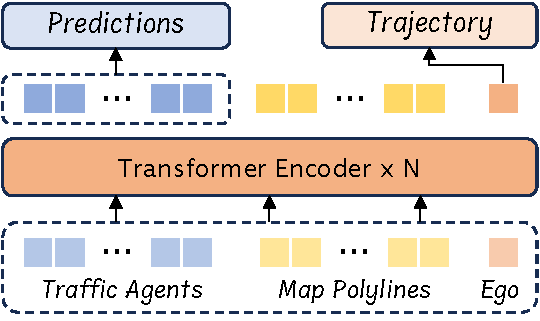
\includegraphics[width=0.65\linewidth]{pics/planning_model.pdf}
    \vspace{-0.5em}
    \caption{基线模型总览。智能体、地图与自车特征分别编码后拼接，再交由堆叠的 Transformer 编码器层处理。基线模型在场景层面联合预测交通智能体，并为自车规划轨迹。}
    \label{fig:baseline_model}
\vspace{-0.5em}
\end{figure}

本文研究采用学习型规划器进行城市导航（urban navigation）的任务，规划器通过模仿数据集中的专家轨迹（expert trajectory）进行训练。每次规划迭代，规划器接收多种输入，包括周围物体最近 2 秒历史窗口的跟踪数据（tracking data）、自车当前与过去的运动学状态、交通信号灯（traffic lights）信息、高清（High-Definition, HD）地图、限速（speed limits）以及指定路线（designated route）。规划器需生成未来 8 秒的轨迹。需要说明的是，除非另有说明，本文直接使用规划器未经修改的轨迹输出，刻意避免规则式紧急停车或后优化（post-optimization）等提升性能的技术，以评估规划器的固有性能。

\paragraph{nuPlan}~\cite{caesar2021nuplan} 是面向自动驾驶车辆的大规模基于机器学习的闭环规划基准测试。该数据集包含从四个城市中心采集的 1300 小时记录驾驶数据，并通过自动化标注工具划分为 75 种场景类型（scenario types）。

\paragraph{仿真}
本文使用 nuPlan 的闭环仿真器作为仿真环境。每次仿真以 10 Hz 的频率推演（rollout）15 秒，采用 LQR 控制器（LQR controller）进行轨迹跟踪（trajectory tracking），控制指令（control commands）通过内部运动学自行车模型（kinematic bicycle model）更新自动驾驶车辆的状态。背景交通（background traffic）的行为随仿真模式而变化，模式可为非反应式（non-reactive，日志回放（log-replay））或反应式（reactive）。

\begin{table*}
\vspace{6pt}
\begin{center}
\setlength{\tabcolsep}{10pt}
\renewcommand{\arraystretch}{1.2}
\small
\begin{tabular}{y{50}y{85}|x{35}x{35}x{35}|x{35}x{35}x{35}}
\toprule
\multicolumn{2}{c}{模型} & \multicolumn{3}{c}{Test14-random} & \multicolumn{3}{c}{Test14-hard} \\ \midrule
输入特征 & \multicolumn{1}{l|}{变体} & OLS & NR-CLS & \multicolumn{1}{c|}{R-CLS} & OLS & NR-CLS & R-CLS \\ \midrule
\multirow{2}{*}{含历史} & \multicolumn{1}{l|}{共享编码器} & 90.20 & 56.50 & \multicolumn{1}{c|}{56.28} & \textbf{88.25} & 48.60 & 51.32 \\
 & \multicolumn{1}{l|}{分离编码器} & \textbf{90.28} & 61.02 & \multicolumn{1}{c|}{59.85} & 86.77 & 51.98 & 49.34 \\ \midrule
\multirow{5}{*}{无历史} & \multicolumn{1}{l|}{state3 (x, y, yaw)} & 81.13 & \textbf{85.99} & \multicolumn{1}{c|}{\textbf{79.38}} & 71.43 & 68.44 & \textbf{63.14} \\
 & \multicolumn{1}{l|}{state4 (+vel.)} & 86.42 & 81.32 & \multicolumn{1}{c|}{75.75} & 82.30 & 68.15 & 62.51 \\
 & \multicolumn{1}{l|}{staet5 (+acc.)} & 87.71 & 81.76 & \multicolumn{1}{c|}{74.51} & 84.54 & \textbf{68.67} & 54.91 \\
 & \multicolumn{1}{l|}{state6 (+steer)} & 88.45 & 83.32 & \multicolumn{1}{c|}{77.52} & 85.93 & 65.15 & 55.99 \\ \bottomrule
\end{tabular}
\end{center}
\vspace{0.5em}
\caption{不同输入特征的结果。对含历史输入的模型，``共享"和``分离"编码器分别表示智能体和自车使用同一历史编码器还是各自独立的编码器。对无历史输入的模型，$+$ 表示与表中前一模型相比增加了一个状态变量。\underline{数值越高}表示各项指标性能越好，最佳结果以\textbf{加粗}标出。}
\label{tab:ego_features}
\vspace{-0.5em}
\end{table*}

\paragraph{评估指标}
本文采用 nuPlan 提供的官方评估指标，包括开环分数（Open-Loop Score, OLS）、非反应式闭环分数（Non-Reactive Closed-Loop Score, NR-CLS）和反应式闭环分数（Reactive Closed-Loop Score, R-CLS）。R-CLS 与 NR-CLS 的计算方法完全相同，唯一区别在于 R-CLS 在仿真中通过智能驾驶模型（Intelligent Driver Model, IDM）~\cite{treiber2000idm}控制背景交通。闭环分数是一个综合性的复合分数，由交通规则遵守（traffic rule adherence）、与人类驾驶相似度（human driving resemblance）、车辆动力学（vehicle dynamics）、目标达成（goal attainment）及场景特定指标等因素加权组合而成，分值范围为 0 至 100。指标的具体定义与计算详见 \cite{nuplan2023metrics}。

\paragraph{基线模型}
作为基线，本文将此前工作~\cite{cheng2023forecast}中的运动预测（motion-forecasting）主干模型改编用于规划任务。图 \ref{fig:baseline_model} 给出了基线模型的简要总览。尽管结构简洁，该架构主要由多个 Transformer 编码器~\cite{vaswani2017attention}构成，展现出强大的建模能力。详细内容请参阅代码库。

\paragraph{基准测试}
所有实验统一采用标准化的训练与评估数据划分。训练阶段使用 nuPlan 训练集中全部 75 种场景类型，场景总数限制为 1M 帧。评估阶段使用 nuPlan 规划挑战赛（Planning Challenge）规定的 14 种场景类型，每种类型包含 20 个场景。本文考察两种场景选取方案：（1）\textbf{Test14-random}：从每种类型中随机采样场景，选定后固定不变；（2）\textbf{Test14-hard}：为考察规划器在长尾场景上的性能，使用最先进的基于规则的规划器（PDM-Closed~\cite{Dauner2023CORL}）运行每种类型的 100 个场景，然后选取每种类型中性能最差的 20 个场景。示例场景见项目主页。由于在线排行榜已停止提交，所有评估均在 nuPlan 公共测试集上进行。

\subsection{输入特征至关重要}
本节旨在回答以下问题：（1）\textit{历史运动数据对规划是否必不可少？}（2）\textit{若不需要，自动驾驶车辆的所有当前状态是否都有助于提升规划器性能？}为此，本文在基线模型基础上构建了两组变体进行探究，结果见表 \ref{tab:ego_features}（Test14-random 与 Test14-hard 基准）。两种含历史输入的变体中，一种与其他交通智能体共享历史编码器，另一种为自车的过去运动使用独立的历史编码器。对仅含状态的模型，本文考察了传统规划器必需的若干关键状态变量，包括车辆位姿、速度、加速度和转向角（steering angle）。基于实验结果，得出以下结论：

\begin{figure}
    \centering
    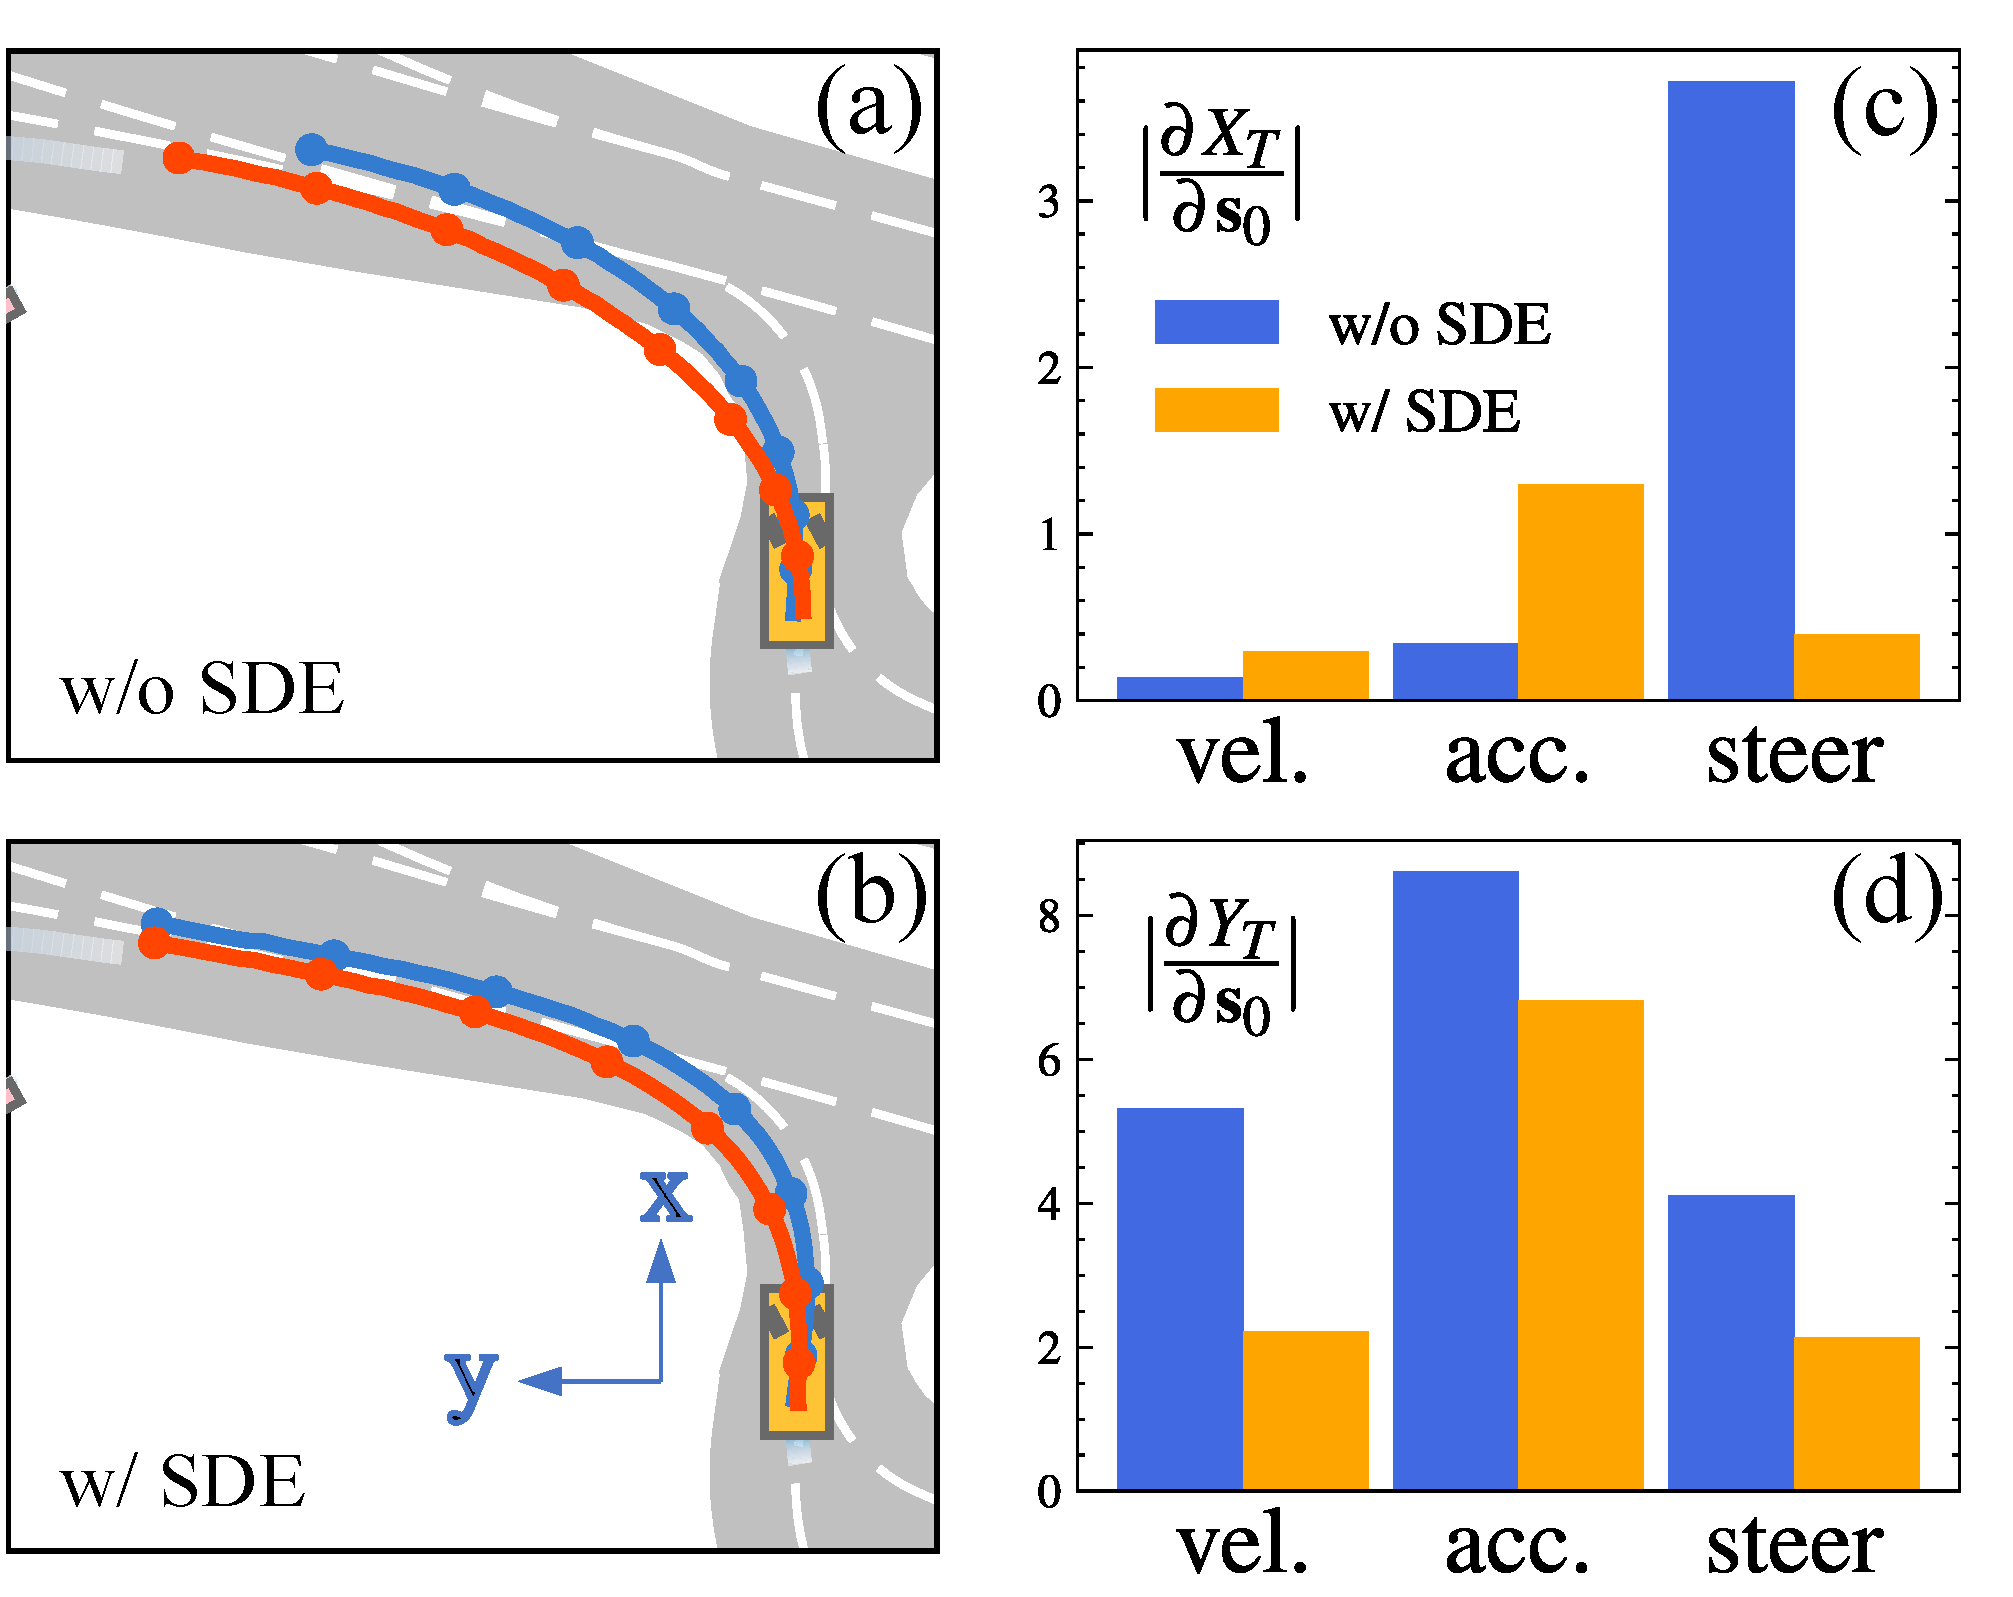
\includegraphics[width=1.0\linewidth]{pics/sense.pdf}
    \vspace{-1em}
    \caption{左侧展示了 \textit{state6} 模型将 AV 转向角从 \textcolor{blue}{0.15} 调整至 \textcolor{red}{0.5} 弧度时的规划轨迹；右侧展示了轨迹终点位置关于 AV 各运动学状态的梯度幅值。}
    \label{fig:left_turn_case}
    % \vspace{-0.5em}
\end{figure}

\begin{figure}
    \centering
    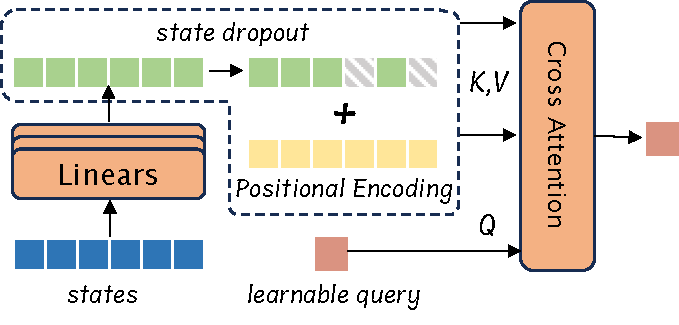
\includegraphics[width=0.75\linewidth]{pics/state_attn_dropout.pdf}
    \vspace{-1em}
    \caption{基于注意力的状态丢弃编码器示意图。}
    \label{fig:state_dropout}
\vspace{-1em}
\end{figure}

\paragraph{历史并非必需}
尽管含历史运动数据的模型在离策略评估（off-policy evaluation）性能（OLS）上表现更优，但其闭环指标明显逊于仅含状态的模型。这一现象可能源于著名的``复制问题（copycat）''~\cite{wen2020fighting}或学习捷径~\cite{geirhos2020shortcut}，即规划器依赖历史数据外推，而未充分理解底层因果因素。此外，随着仅含状态模型的状态数量增加，含历史模型的开环性能优势迅速缩小。因此，本文认为历史运动对规划模型并非必需。

\begin{table*}[h!]
\begin{center}
\setlength{\tabcolsep}{5pt}
\renewcommand{\arraystretch}{1.2}
\small
\begin{tabular}{y{25}x{30}y{50}y{60}x{60}y{50}y{60}y{60}}
\toprule
 &  & \multicolumn{3}{c}{Test14-random} & \multicolumn{3}{c}{Test14-hard} \\ \midrule
 & \multicolumn{1}{c|}{SDE} & OLS & NR-CLS & \multicolumn{1}{l|}{R-CLS} & OLS & NR-CLS & R-CLS \\ \midrule
\fadedtext{staet3} & \multicolumn{1}{c|}{-} & \fadedtext{81.13} & \fadedtext{85.99} & \multicolumn{1}{l|}{\fadedtext{79.38}} & \fadedtext{71.43} & \fadedtext{68.44} & \fadedtext{63.14} \\ \midrule
\multirow{2}{*}{state5} & \multicolumn{1}{c|}{\xmark} & 87.71 & 81.76 & \multicolumn{1}{l|}{74.51} & 84.54 & 68.67 & 54.91 \\
 & \multicolumn{1}{c|}{\cmark} & 88.80 \textcolor{blue}{(+1.09)} & 86.73 \textcolor{blue}{(+4.97)} & \multicolumn{1}{l|}{75.75 \textcolor{blue}{(+1.24)}} & 84.29 \textcolor{red}{(-0.25)} & 71.28 \textcolor{blue}{(+2.61)} & 61.88 \textcolor{blue}{(+6.97)} \\ \midrule
\multirow{2}{*}{state6} & \multicolumn{1}{c|}{\xmark} & 88.55 & 83.19 & \multicolumn{1}{l|}{74.79} & 85.89 & 67.57 & 58.99 \\
 & \multicolumn{1}{c|}{\cmark} & 87.07 \textcolor{red}{(-1.48)} & 86.48 \textcolor{blue}{(+3.29)} & \multicolumn{1}{l|}{80.59 \textcolor{blue}{(+5.80)}} & 83.32 \textcolor{red}{(-2.57)} & 72.68 \textcolor{blue}{(+5.11)} & 61.70 \textcolor{blue}{(+2.71)} \\ \bottomrule
\end{tabular}
\end{center}
\vspace{0.5em}
\caption{状态丢弃编码器（State Dropout Encoder, SDE）在 Test14-random 与 Test14-hard 基准上的实验结果。使用 SDE 的模型在闭环分数（CLS）上获得显著提升，同时保持较高的 OLS。}
\label{tab:state_dropout}
\vspace{-1em}
\end{table*}

\paragraph{运动学状态中的捷径学习}
速度、加速度等运动学状态是轨迹规划中保证安全与舒适的关键初始边界条件（boundary conditions）。然而，本文意外发现，仅依赖 AV 位姿（位置与航向）的 \textit{state3} 模型在闭环分数指标上显著优于其他含运动学状态的模型。为深入理解该现象，本文研究了 \textit{state6} 模型的一个左转案例。如图 \ref{fig:left_turn_case}\textcolor{red}{a} 所示，将转向角从 0.15（蓝色）调整为 0.5（红色）弧度时，模型生成了不期望的偏离道路轨迹（off-road trajectory）。本文推测，即使没有历史观测，模型仍可能从运动学信息中学习到虚假的相关关系。

\paragraph{状态丢弃编码器}
为验证上述推测，本文提出基于注意力的状态丢弃编码器（State Dropout Encoder, SDE），如图 \ref{fig:state_dropout} 所示。每个状态变量先经线性层（linear layer）独立嵌入，再与位置编码（positional encoding）相加；可学习查询（learnable query）通过交叉注意力（cross-attention）模块聚合各状态嵌入。训练时，每个已嵌入的状态（位置与航向除外）以一定概率被丢弃。该编码器通过部分限制模型对辅助信息的访问，迫使模型揭示行为的根本成因；同时，当运动学属性可用时，模型仍能增强规划能力。本文将状态丢弃编码器应用于 \textit{state5} 与 \textit{state6} 模型，结果见表 \ref{tab:state_dropout}。结果表明，使用 SDE 显著提升了模型的闭环性能。更重要的是，与 \textit{state3} 相比，加入 SDE 的 \textit{state5} 和 \textit{state6} 模型不仅闭环分数更高，开环分数也大幅提升，为 SDE 的有效性提供了有力证据。需要指出的是，\textit{state3} 模型本质上存在歧义——它丢失了全部运动学信息（其较差的 OLS 性能即是佐证）。图
\ref{fig:left_turn_case}(a)(b) 展示了 \textit{state6} 模型的规划结果对比，图 \ref{fig:left_turn_case}(c)(d) 则展示了终点位置 $(X_T, Y_T)$ 相对于初始运动学状态 $s_0$ 的梯度幅值对比。结果表明，采用 SDE 的模型对运动学状态的变化更不敏感，规划结果更具鲁棒性。

\begin{figure}
    \centering
    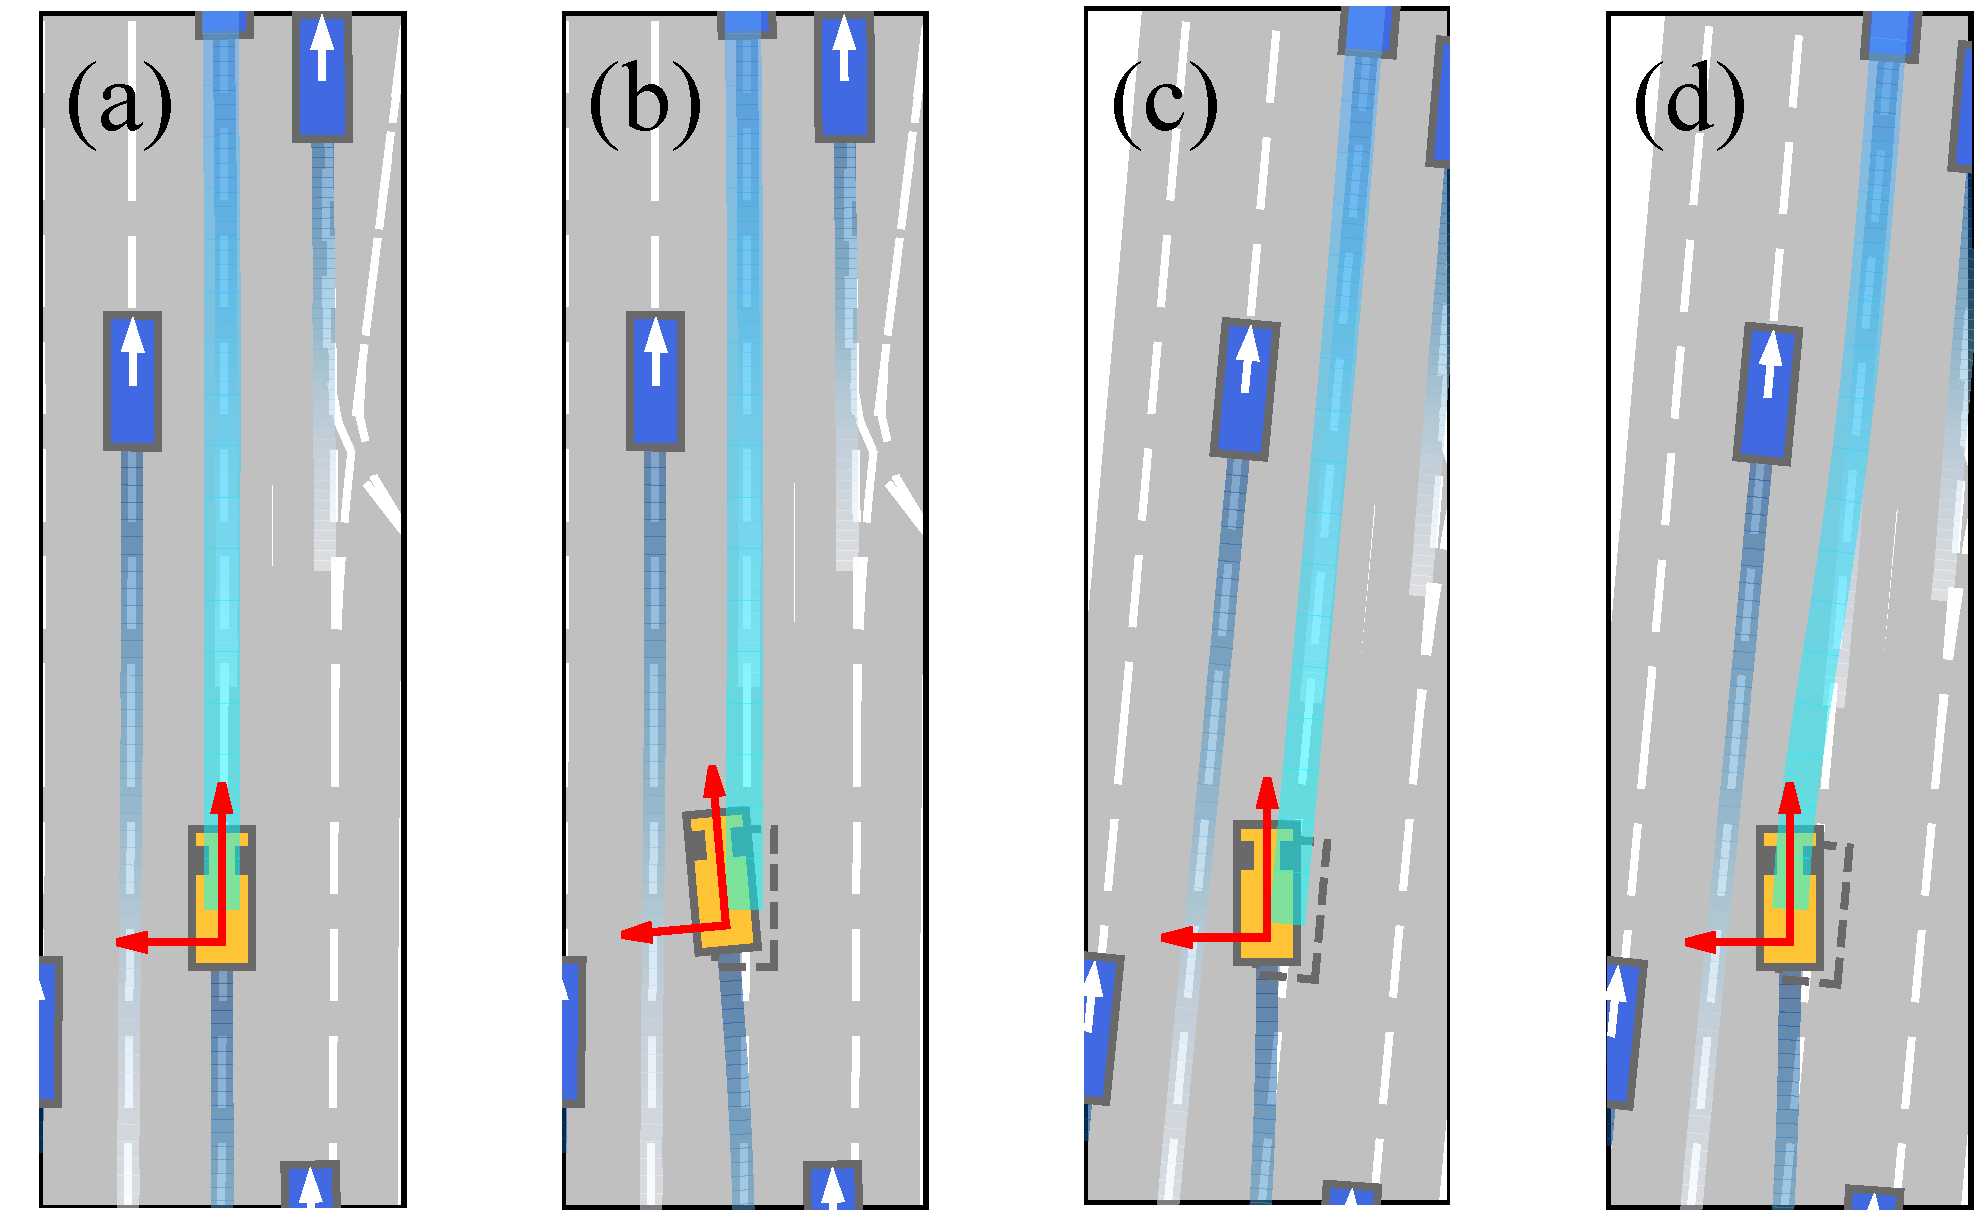
\includegraphics[width=0.75\linewidth]{pics/aug_vis.pdf}
    \vspace{-0.5em}
    \caption{（a）原始场景。（b）对 AV 当前状态添加随机噪声，并平滑历史运动。（c）根据 AV 扰动后的位置对场景坐标进行重新归一化（re-normalization）。（d）通过约束非线性优化生成修正后的未来轨迹。 }
    \label{fig:aug_vis}
\end{figure}

\begin{table}[!h]
\begin{center}
\setlength{\tabcolsep}{5pt}
\renewcommand{\arraystretch}{1.2}
\small
\begin{tabular}{y{25}x{10}x{15}x{15}|x{30}x{35}x{30}}
\toprule
 & P & RN & FC & OLS & NR-CLS & R-CLS \\ \midrule
\multirow{2}{*}{history} & \xmark & \xmark & \xmark & 88.99 & 65.84 & 65.58 \\
 & \cmark & \cmark & \cmark & 89.94 & 65.14 & 66.03 \\ \midrule
\multirow{4}{*}{state3} & \xmark & \xmark & \xmark & 78.92 & 71.86 & 70.87 \\
 & \cmark & \xmark & \xmark & 80.85 & 74.28 & 71.69 \\
 & \cmark & \cmark & \xmark & 81.13 & 85.99 & 79.38 \\
 & \cmark & \cmark & \cmark & 79.28 & 81.35 & 76.60 \\ \midrule
\multirow{4}{*}{state5} & \xmark & \xmark & \xmark & 88.44 & 80.67 & 74.50 \\
 & \cmark & \xmark & \xmark & 89.20 & 79.85 & 72.43 \\
 & \cmark & \cmark & \xmark & 87.71 & 81.76 & 74.51 \\
 & \cmark & \cmark & \cmark & 86.43 & 82.10 & 74.71 \\ \midrule
\multicolumn{1}{c}{\multirow{4}{*}{\begin{tabular}[c]{@{}c@{}}state6\\ +SDE\end{tabular}}} & \xmark & \xmark & \xmark & 88.33 & 77.28 & 74.10 \\
\multicolumn{1}{c}{} & \cmark & \xmark & \xmark & 87.71 & 77.70 & 75.18 \\
\multicolumn{1}{c}{} & \cmark & \cmark & \xmark & 87.07 & 86.48 & 80.59 \\
\multicolumn{1}{c}{} & \cmark & \cmark & \cmark & 85.50 & 82.95 & 76.09 \\ \bottomrule
\end{tabular}
\end{center}
\caption{在 \textbf{Test14-random} 基准上不同增强与归一化组合的结果。P：\textbf{P}erturbation（扰动）；RN：\textbf{R}e-\textbf{N}ormalization（重新归一化）；FC：\textbf{F}uture \textbf{C}orrection（未来轨迹修正）。}
\label{tab:aug}
\vspace{-2em}
\end{table}

\subsection{数据增强与归一化}

数据增强是基于 IL 的模型学习从偏差中恢复的常用手段。本节对不同的数据增强技术进行全面实验，探索缓解复合误差的有效策略，各增强策略如图 \ref{fig:aug_vis} 所示。图 \ref{fig:aug_vis}(a) 是一个示例驾驶场景，所有坐标均以自动驾驶车辆中心为基准归一化。图 \ref{fig:aug_vis}(b) 中，对 AV 当前状态添加随机采样的噪声（扰动），并相应平滑其历史状态。图 \ref{fig:aug_vis}(c) 表明，扰动后场景坐标以自动驾驶车辆中心为基准重新归一化。图 \ref{fig:aug_vis}(d) 展示了通过非线性优化生成修正的未来轨迹。本质上，图 \ref{fig:aug_vis}(b) 与 \ref{fig:aug_vis}(d) 两种策略的目标一致，都是引导车辆回到专家轨迹。

表 \ref{tab:aug} 展示了四种模型变体在不同增强策略下的实验结果。基于这些结果，得出以下结论：（1）对 \textit{history} 和 \textit{state5} 模型，各种数据增强均未带来显著提升。本文推测这两个模型面临的主要挑战是因果混淆（causal confusion）问题，即从历史状态或运动学状态进行外推。（2）对 \textit{state3} 和 \textit{state6+SDE} 模型，扰动至关重要，但仅在恰当的归一化下才有效。例如，\textit{state3} 模型在扰动加重新归一化下 NR-CLS 从 71.86 提升至 85.99，远高于仅使用扰动时的 74.28。这表明保持训练与测试数据分布接近十分重要。（3）提供修正后的引导未来轨迹并无正面效果。一个可能的原因是手工生成的轨迹与专家轨迹分布不一致。直接以专家轨迹作为监督（supervision）是更有效的选择，因为这保持了原始分布，且小的偏差易于由轨迹跟踪器纠正。

\begin{figure}
    \centering
    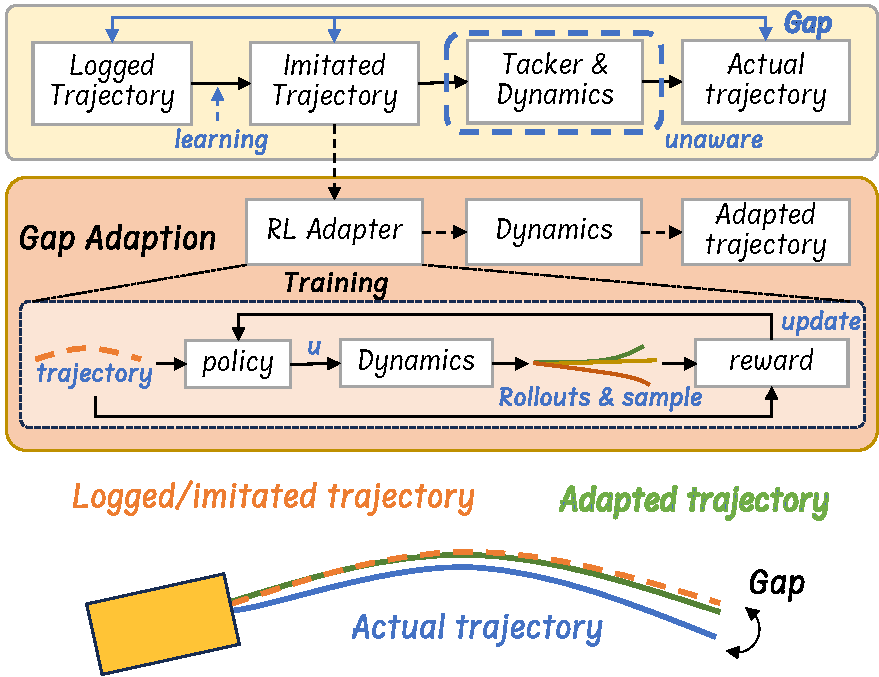
\includegraphics[width=0.9\linewidth]{pics/imitation_gap.pdf}
    \caption{模仿差距与所提出的强化学习适配器（RL Adapter）示意图。 }
    \label{fig:imitatoin_gap}
\end{figure}

\begin{table}[]
\begin{center}
\setlength{\tabcolsep}{5pt}
\renewcommand{\arraystretch}{1.2}
\small
\begin{tabular}{y{60}x{35}x{30}|x{35}x{30}}
\toprule
                                      & \multicolumn{2}{c}{Test14-random}   & \multicolumn{2}{c}{Test14-hard} \\ \midrule
\multicolumn{1}{l|}{Log-replay +}          & NR-CLS & \multicolumn{1}{c|}{R-CLS} & NR-CLS          & R-CLS         \\ \midrule
\multicolumn{1}{l|}{\fadedtext{Perfect tracking}} & \fadedtext{96.63}  & \multicolumn{1}{c|}{\fadedtext{77.38}} & \fadedtext{91.61}           & \fadedtext{71.34}         \\ \midrule
\multicolumn{1}{l|}{LQR}              & 94.03  & \multicolumn{1}{c|}{75.86} & 85.96           & 68.80          \\
\multicolumn{1}{l|}{RL Adapter}       & 96.3   & \multicolumn{1}{c|}{77.13} & 91.65           & 71.62         \\ \bottomrule
\end{tabular}
\end{center}
\vspace{0.5em}
\caption{日志回放规划器（log-replay planner，完美模仿）配合不同轨迹跟踪器在 Test14-random 与 Test14-hard 基准上的实验结果。LQR 是 nuPlan 基准测试使用的默认跟踪器，RL 适配器是本文为解决模仿差距提出的方法。}
\label{tab:il_gap}
\vspace{-1em}
\end{table}

\subsection{隐性的模仿差距}

\paragraph{模仿差距} 在主流模仿学习框架中，模型模仿数据集中记录的专家轨迹。本文认为，这种学习框架会导致隐性的模仿差距，可能造成显著的性能下降。如图 \ref{fig:imitatoin_gap} 所示，记录轨迹即专家轨迹，在基于模仿的规划器训练中充当真值（ground truth）。生成的模仿轨迹随后经下游轨迹跟踪器和底层系统动力学处理，得到 AV 的最终轨迹。然而，由于训练时对跟踪器和动力学一无所知，即使模仿完美无瑕，实际轨迹仍可能与记录轨迹产生显著偏差。表 \ref{tab:il_gap} 的实验结果支持了这一论断：在 Test14-hard 上，\textit{Log-replay + LQR} 方法的 NR-CLS 相比完美跟踪（perfect tracking）显著下降了 $5.65$。

\begin{table}
\begin{center}
\setlength{\tabcolsep}{5pt}
\renewcommand{\arraystretch}{1.1}
\small
\begin{tabular}{y{70}x{70}x{60}}
\toprule
奖励项       & 表达式 & 权重 \\ \midrule
位置跟踪 & $e^{-15||\mathbf{p}_{xy}-\mathbf{p}^*_{xy}||}$ &  1.0     \\
动作            & $||\mathbf{u}||^2$ & -0.01    \\
动作变化率       & $||\dot{\mathbf{u}}||^2$ & -0.1     \\
纵向加速度限制   & $\mathbb{1}({\dot{v}}>2.4)$ & -1    \\
加加速度限制        & $\mathbb{1}(||{\ddot{v}}||>4.0)$  & -1        \\
横摆角速度          & $\mathbb{1}(||{\dot{\theta}}||>0.95)$ & -0.5        \\ \bottomrule
\end{tabular}
\end{center}
\vspace{0.5em}
\caption{RL 适配器的奖励项（reward terms）与表达式。动作 $\mathbf{u}$ 包含加速度和转向速率。$v$ 与 $\theta$ 分别指 AV 的纵向（longitudinal）速度与航向角（heading angle）。}
\label{tab:rewards}
\vspace{-1em}
\end{table}

\begin{table*}[]
\vspace{6pt}
\begin{center}
\setlength{\tabcolsep}{10pt}
\renewcommand{\arraystretch}{1.2}
\small
\begin{tabular}{y{58}y{70}|x{25}x{33}x{30}|x{25}x{33}x{30}x{30}}
\toprule
\multicolumn{2}{c}{规划器} & \multicolumn{3}{c}{Test14-random} & \multicolumn{3}{c}{Test14-hard} &  \\ \midrule
类型 & \multicolumn{1}{l|}{方法} & OLS & NR-CLS & \multicolumn{1}{c|}{R-CLS} & OLS & NR-CLS & \multicolumn{1}{c|}{R-CLS} & 时间(ms) \\ \midrule
\fadedtext{专家} & \multicolumn{1}{l|}{\fadedtext{日志回放}} & \fadedtext{100.0} & \fadedtext{94.03} & \multicolumn{1}{c|}{\fadedtext{75.86}} & \fadedtext{100.0} & \fadedtext{85.96} & \multicolumn{1}{c|}{\fadedtext{68.80}} & \fadedtext{-} \\ \midrule
\multirow{2}{*}{基于规则} & \multicolumn{1}{l|}{IDM~\cite{treiber2000idm}} & 34.15 & 70.39 & \multicolumn{1}{c|}{72.42} & 20.07 & 56.16 & \multicolumn{1}{c|}{62.26} & 32 \\
 & \multicolumn{1}{l|}{PDM-Closed~\cite{Dauner2023CORL}} & 46.32 & 90.05 & \multicolumn{1}{c|}{\textbf{91.64}} & 26.43 & 65.07 & \multicolumn{1}{c|}{75.18} & 140 \\ \midrule
\multirow{2}{*}{混合$^\dagger$} & \multicolumn{1}{l|}{GameFormer~\cite{huang2023gameformer}} & 79.35 & 80.80 & \multicolumn{1}{c|}{79.31} & 75.27 & 66.59 & \multicolumn{1}{c|}{68.83} & 443 \\
 & \multicolumn{1}{l|}{PDM-Hybrid~\cite{Dauner2023CORL}} & 82.21 & \textbf{90.20} & \multicolumn{1}{c|}{91.56} & 73.81 & 65.95 & \multicolumn{1}{c|}{\textbf{75.79}} & 152 \\ \midrule
\multirow{5}{*}{基于学习} & \multicolumn{1}{l|}{RasterModel~\cite{caesar2021nuplan}} & 62.93 & 69.66 & \multicolumn{1}{c|}{67.54} & 52.4 & 49.47 & \multicolumn{1}{c|}{52.16} & 82 \\
 & \multicolumn{1}{l|}{UrbanDriver~\cite{scheel2022urban}} & 82.44 & 63.27 & \multicolumn{1}{c|}{61.02} & 76.9 & 51.54 & \multicolumn{1}{c|}{49.07} & 124 \\
 & \multicolumn{1}{l|}{GC-PGP~\cite{hallgarten2023gc-pgp}} & 77.33 & 55.99 & \multicolumn{1}{c|}{51.39} & 73.78 & 43.22 & \multicolumn{1}{c|}{39.63} & 160 \\
 & \multicolumn{1}{l|}{PDM-Open~\cite{Dauner2023CORL}} & 84.14 & 52.80 & \multicolumn{1}{c|}{57.23} & 79.06 & 33.51 & \multicolumn{1}{c|}{35.83} & 101 \\
 & \multicolumn{1}{l|}{PlanTF (本文)} & \textbf{87.07} & 86.48 & \multicolumn{1}{c|}{80.59} & \textbf{83.32} & \textbf{72.68} & \multicolumn{1}{c|}{61.7} & 155 \\ \bottomrule
\end{tabular}
\end{center}
\caption{与最先进方法的对比。运行时间包括基于 Python 代码的特征提取和模型推理。\\\textit{\footnotesize $^\dagger$ 表示这些方法的最终输出轨迹依赖基于规则的策略或后优化。}}
\label{tab:sota}
\vspace{-1em}
\end{table*}

\paragraph{强化学习适配器} 一种可能的方案是直接模仿控制指令（control command）而非轨迹点。然而，该方法严重依赖具体的车辆模型，其泛化性和可解释性不如基于轨迹的方法。另一种方案是在轨迹解码器中引入可微（differentiable）运动学模型~\cite{cui2020deep,zhou2021exploring}，但为保证可微性，运动学模型往往被过度简化。为解决这一问题，本文提出一种基于强化学习的轨迹适配器（RL Adapter）来弥合这一差距。RL 适配器在考虑底层动力学的前提下，将模仿轨迹转换为相应的控制指令。其优势有二：一是无需重新训练规划器即可适配多种车辆模型；二是对车辆模型不作任何约束，兼容不可微的车辆模型（例如高保真（high-fidelity）真实车辆动力学模型）。适配器的训练过程见图 \ref{fig:imitatoin_gap}，奖励设置见表 \ref{tab:rewards}。本文使用近端策略优化（Proximal Policy Optimization, PPO）~\cite{schulman2017proximal} 进行策略优化，训练在 8 万步内完成，学习率为 1e-3。如表 \ref{tab:il_gap} 所示，RL 适配器的表现与完美跟踪相当，展现了其弥合模仿差距的能力。值得注意的是，该适配器可以融入规划器的训练过程，本文将其留作未来工作。

\section{与最先进方法的比较}

\paragraph{实现细节}
综合本文研究发现，本文提出一个完全基于学习的基线规划模型——规划 Transformer（Planning Transformer, \textbf{PlanTF}）。具体而言，采用 \textit{state6} 模型，并集成丢弃率（dropout rate）为 0.75 的状态注意力丢弃编码器。训练时以 0.5 的概率施加状态扰动。模型以批大小（batch size）128、权重衰减（weight decay）1e-4 训练 25 轮。初始学习率（learning rate）设为 1e-3，按余弦方式（cosine manner）衰减至零。

\paragraph{对比方法}
本文将 PlanTF 与若干最先进的规划器进行比较。（1）\textbf{RasterModel} 是~\cite{caesar2021nuplan}提供的基于 CNN 的规划器。（2）\textbf{UrbanDriver}~\cite{scheel2022urban} 是基于 PointNet 的折线编码器（polyline encoders）与 Transformer 的矢量化规划器。此处使用其开环重实现，训练时采用历史扰动。（3）\textbf{GameFormer}~\cite{huang2023gameformer} 是基于 level-k 博弈（level-k game）的 DETR 式（DETR-like）交互式预测与规划框架，并引入后优化器生成最终轨迹。（4）\textbf{PDM*}~\cite{Dauner2023CORL} 是 2023 年 nuPlan 规划挑战赛的获胜方案。\textbf{PDM-Closed} 是完全基于规则的方法，对不同超参数的 IDM~\cite{treiber2000idm}进行集成。\textbf{PDM-Hybrid} 是 PDM-Closed 的变体，增加偏移预测器以提升其开环预测性能。\textbf{PDM-Open} 是不含基于 IDM 规划器的纯学习组件。上述结果均使用其公开代码复现，并在本文标准的 1M 数据划分上训练。

\paragraph{实验结果}
表 \ref{tab:sota} 给出了 Test14-random 与 Test14-hard 基准上的对比结果。首先，本文提出的 PlanTF 在所有指标上显著优于其他纯基于模仿的方法，尤其是闭环性能；它也是唯一超越公认 IDM 的基于学习的方法，凸显了 IL 中恰当设计的重要性。其次，与基于规则和混合方法相比，PlanTF 在保持极具竞争力的闭环分数的同时实现了出色的 OLS，且无需任何精巧的手工规则或策略。值得注意的是，本文方法在 Test14-hard 基准上取得了最高的 NR-CLS，说明基于规则的方法在常规场景（Test14-random）中表现良好，但在长尾情形（Test14-hard）中泛化能力不足；相比之下，PlanTF 展现出更强的泛化能力。

\section{结论}

本文利用标准化的 nuPlan 基准，系统考察了基于模仿的规划器若干关键设计方面。研究发现，历史运动和单帧运动学状态等输入特征普遍存在灾难性的捷径学习问题，这导致了一个反直觉的结果：仅基于 AV 当前位置进行规划反而取得更优的闭环性能。为缓解该问题，本文提出简单有效的基于注意力的状态丢弃编码器（SDE），有效解决了捷径学习问题；引入 SDE 后，\textit{state6} 模型取得了最佳整体性能。数据增强是基于模仿的规划器的另一个重要因素。结果表明，扰动对减少复合误差至关重要，但仅在恰当的特征归一化下才有效；此外，即使经过扰动，原始专家轨迹仍是可靠的训练真值。除上述发现外，本文还识别出一个被忽视的模仿差距——模型对底层系统动力学缺乏感知，这会显著影响规划器性能。为弥补这一差距，本文提出基于强化学习的适配器。结合全部研究发现，本文提出的纯基于学习的基线模型 PlanTF 相比最先进方法表现出色，与采用复杂基于规则策略或后优化的方法不相上下，凸显了基于模仿学习的规划器中恰当设计选择的重要性。

\paragraph{局限性与未来工作}
尽管本文方法拓展了纯基于模仿规划器的边界，但仍受限于\textit{开环训练}与\textit{闭环测试}之间的根本性不匹配。将闭环信息和系统动力学纳入训练过程是未来的研究方向。

\appendix

\paragraph{Val14 基准上的附加结果} 本文在 \textbf{Val14}~\cite{Dauner2023CORL} 基准上给出了对比结果（表 \ref{tab:val14}）。\textbf{Val14} 包含来自 14 种场景类型的 1180 个场景。

\begin{table}[h]
\vspace{6pt}
\begin{center}
\setlength{\tabcolsep}{7pt}
\renewcommand{\arraystretch}{1.2}
\small
\begin{tabular}{y{70}|x{30}x{35}x{30}}
\toprule
方法       & OLS & NR-CLS & R-CLS \\ \midrule
\fadedtext{Log-replay}   & \fadedtext{100} & \fadedtext{94}     & \fadedtext{80}    \\
IDM~\cite{treiber2000idm}          & 38  & 77     & 76    \\
GC-PGP~\cite{hallgarten2023gc-pgp}       & 82  & 57     & 54    \\
PlanCNN~\cite{caesar2021nuplan}      & 64  & 73     & 72    \\
PDM-Hybrid~\cite{Dauner2023CORL}   & 84  & 93     & 92    \\ \midrule
PlanTF (本文) & 89.18    & 84.83  & 76.78 \\ \bottomrule
\end{tabular}
\end{center}
\vspace{0.5em}
\caption{在 Val14 基准上与最先进方法的对比。其他方法的结果取自~\cite{Dauner2023CORL}。}
\label{tab:val14}
\end{table}

\paragraph{状态丢弃率消融实验} 表 \ref{tab:abl_dropout} 展示了 \textit{state6+SDE} 模型在不同状态丢弃率下的消融实验（ablation study）。

\begin{table}[h]
\vspace{6pt}
\begin{center}
\setlength{\tabcolsep}{6pt}
\renewcommand{\arraystretch}{1.2}
\small
\begin{tabular}{y{30}|x{30}|x{35}x{35}x{30}}
\toprule
模型                   & \multicolumn{1}{l|}{丢弃率} & OLS   & NR-CLS & R-CLS \\ \midrule
\multirow{4}{*}{state6} & -                          & 88.33 & 77.28  & 74.10 \\
                        & 0.25                         & 89.11 & 81.70  & 78.44 \\
                        & 0.50                         & 89.12 & 83.71  & 77.52 \\
                        & 0.75                         & 87.07 & 86.48  & 80.59 \\ \bottomrule
\end{tabular}
\end{center}
\vspace{0.5em}
\caption{SDE 状态丢弃率的消融实验。}
\label{tab:abl_dropout}
\end{table}
% \clearpage
% \newpage
% \addtolength{\textheight}{-12cm}   % This command serves to balance the column lengths
                                  % on the last page of the document manually. It shortens
                                  % the textheight of the last page by a suitable amount.
                                  % This command does not take effect until the next page
                                  % so it should come on the page before the last. Make
                                  % sure that you do not shorten the textheight too much.

%%%%%%%%%%%%%%%%%%%%%%%%%%%%%%%%%%%%%%%%%%%%%%%%%%%%%%%%%%%%%%%%%%%%%%%%%%%%%%%%

\bibliographystyle{IEEEtran}
\bibliography{IEEEabrv,ref}

\end{document}
